\section{Project Management \& Development}
\subsection{Obstacles}
\begin{frame}{Project Management \& Development}
    \begin{itemize}
        \item Version Control
        \begin{itemize}
            \item Manageing repositories and sourcecode
        \end{itemize}
        \item Code Review
        \begin{itemize}
            \item Structuring review process
            \item Easy access to code that needs review
        \end{itemize}
        \item Wiki
        \begin{itemize}
            \item Guides
            \item General GIRAF information
        \end{itemize}
        \item Documentation
        \begin{itemize}
            \item Javadoc
            \item REST API service doc.
        \end{itemize}
        \item Continuous Integration
        \begin{itemize}
            \item Automated build
            \item Test
            \item Deployment to Google Play
        \end{itemize}
        \item Artifact Repository
        \begin{itemize}
            \item Pre--compiled libraries
        \end{itemize}
    \end{itemize}
\end{frame}

\subsection{Tools}
\begin{frame}{Project Management \& Development}\framesubtitle{Version Control}
    \textbf{Git}
    \begin{itemize}
        \item Foundation of the workflow
        \item Gogs
        \begin{itemize}
            \item Restricted to AAU developers
            \item Custom git--hooks
        \end{itemize}
        \item Powerful
        \item Easy to make mistakes
    \end{itemize}
\end{frame}

\begin{frame}{Project Management \& Development}\framesubtitle{Code Review, Wiki}
    \textbf{Phabricator}
    \begin{itemize}
        \item Arcanist
        \begin{itemize}
            \item Uses git
            \item Interfaces with Phabricator
            \item Unit tests \& linting
        \end{itemize}
        \item Web interface
        \begin{itemize}
            \item Hub for the entire multi--project
            \item Code review
            \item User story and task management
            \begin{itemize}
                \item Backlog
                \item Assigning to groups
            \end{itemize}
            \item Scrumboards
            \item Wiki
        \end{itemize}
    \end{itemize}
\end{frame}
\begin{frame}{Project Management \& Development}\framesubtitle{CI, Documentation, Artifact Repo}
    \textbf{Jenkins}
    \begin{itemize}
        \item Gradle
        \begin{itemize}
            \item Build tool
        \end{itemize}
        \item Automated Testing
        \begin{itemize}
            \item Monkey test
            \item Unit tests
        \end{itemize}
        \item Artifactory
        \begin{itemize}
            \item Maven repository
            \item Multiple versions of libraries
        \end{itemize}
        \item Javadoc \& Enunciate
    \end{itemize}
\end{frame}

\section{Architecture}
\subsection{Old GIRAF}
\begin{frame}{Architecture}\framesubtitle{Old GIRAF architecture}
    \only<1>{%
    \centering
    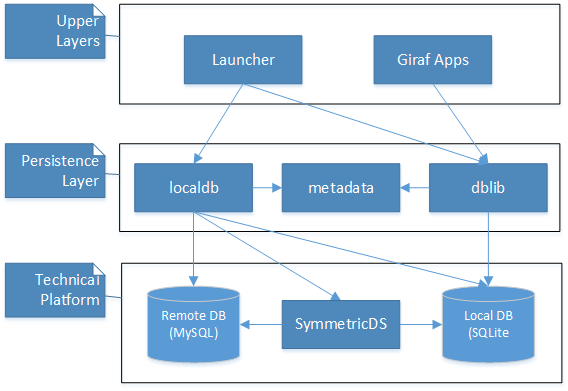
\includegraphics[width=0.8\textwidth]{images/old_architecture.png}}
    \only<2>{%
    \centering
    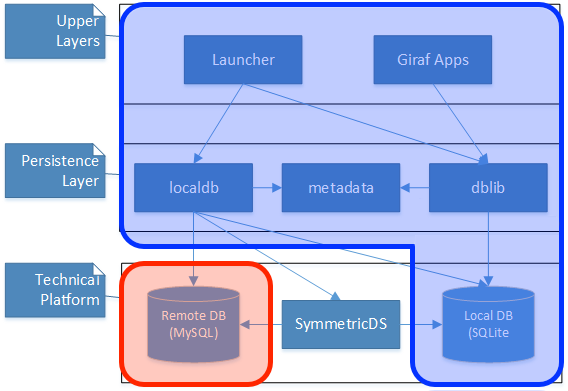
\includegraphics[width=0.8\textwidth]{images/old_architecture_memes.png}}
    \onslide<2->{%
    \begin{itemize}
        \item High coupling
        \item Low cohesion
    \end{itemize}}
\end{frame}

\subsection{New GIRAF}
\begin{frame}{Architecture}\framesubtitle{New GIRAF architecture}
    \begin{columns}
        \hspace{-1.75em}%
        \column{0.55\textwidth}%
        \centering
        \scalebox{0.575}{%
        \pgfdeclarelayer{background}
\pgfsetlayers{background,main}
\tikzstyle{double_arrow}=[latex'-latex']
\tikzstyle{component}=[draw, fill=blue!20, text width=8em,
text centered, minimum height=2.5em]
\tikzstyle{client_comp}=[draw, fill=blue!20, text width=4em,
text centered, minimum height=2.5em]
\tikzstyle{client_comp_synca}=[draw, fill=blue!20, text width=4em,
text centered, minimum height=1.5em]
\tikzstyle{bgbox}=[fill=green!20, rounded corners, draw=GoogleGrey, dashed]
\begin{tikzpicture}[auto]

    %%%%%%%%%%%%%%%%%%%%%%%%%%%%%%%%%%%%%%%%%%%%%%%%%%%%%%%%%%%%%%%%%%%%%
    % REST API                                                          %
    %%%%%%%%%%%%%%%%%%%%%%%%%%%%%%%%%%%%%%%%%%%%%%%%%%%%%%%%%%%%%%%%%%%%%
    \node[component] (persistence) {Persistence};
    \node[component, above = 0.6cm of persistence] (service) {Service};
    %core
    \path (persistence.south -| persistence.east)+(1,0) node (core_a) {};
    \path (service.north -| service.east)+(2,0) node (core_b) {};
    \path[draw, fill = blue!20] (core_a) rectangle (core_b);
    \path ($ (core_a) !.5! (core_b) $) node (core) {Core};

    %REST API background box
    \begin{pgfonlayer}{background}
        % Compute a few helper coordinates
        \path (service.west |- service.north)+(-3,+0.5) node (rest_a) {};
        \path (core_a)+(+2,-0.5) node (rest_b) {};
        \path [bgbox] (rest_a) rectangle (rest_b);
        \node [below = 0.5em of rest_a, anchor = west, inner sep = 0.5em]{REST API};
    \end{pgfonlayer}

    %Awwowwwws
    \draw [<-, dashed] ($(service.south)+(+0.1,0)$) -- ($(persistence.north)+(+0.1,0)$);
    \draw [->]     ($(service.south)+(-0.1,0)$) -- ($(persistence.north)+(-0.1,0)$);
    \draw [->]     (service) -- node {uses} (service -| core_a);
    \draw [->]     (persistence) -- node {uses} (persistence -| core_a);

    %%%%%%%%%%%%%%%%%%%%%%%%%%%%%%%%%%%%%%%%%%%%%%%%%%%%%%%%%%%%%%%%%%%%%
    % Storage                                                           %
    %%%%%%%%%%%%%%%%%%%%%%%%%%%%%%%%%%%%%%%%%%%%%%%%%%%%%%%%%%%%%%%%%%%%%
    \node[component, below = 1.5cm of persistence] (db) {Database};

    \draw [<-, dashed] ($(persistence.south)+(+0.1,0)$) -- ($(db.north)+(+0.1,0)$);
    \draw [->]     ($(persistence.south)+(-0.1,0)$) -- ($(db.north)+(-0.1,0)$);

    %storage background box
    \begin{pgfonlayer}{background}
        % Compute a few helper coordinates
        \path (db.west |- db.north)+(-3,+0.5) node (db_a) {};
        \path (core_a |- db.south)+(+2,-0.5) node (db_b) {};
        \path [bgbox] (db_a) rectangle (db_b);
        \node [below = 0.5em of db_a, anchor = west, inner sep = 0.5em]{Storage};
    \end{pgfonlayer}

    %%%%%%%%%%%%%%%%%%%%%%%%%%%%%%%%%%%%%%%%%%%%%%%%%%%%%%%%%%%%%%%%%%%%%
    % Web 'n' client                                                    %
    %%%%%%%%%%%%%%%%%%%%%%%%%%%%%%%%%%%%%%%%%%%%%%%%%%%%%%%%%%%%%%%%%%%%%
    \node[draw, cloud, cloud puffs=12, cloud ignores aspect, minimum width=9em, minimum height=5em,fill=blue!20, above = 1cm of service](web) {Internet};
    \draw [<-, dashed] ($(web.south)+(+0.1,0)$) -- ($(service.north)+(+0.1,0)$);
    \draw [->]     ($(web.south)+(-0.1,0)$) -- ($(service.north)+(-0.1,0)$);

    % CLIENT GALORE
    \node[client_comp, above = 2cm of web](client2) {$\text{App}_{2}$};
    \node[client_comp_synca, below = 0.3cm of client2] (client2_synca) {S.A.};
    \draw [<-, dashed] ($(client2.south)+(+0.1,0)$) -- ($(client2_synca.north)+(+0.1,0)$);
    \draw [->]     ($(client2.south)+(-0.1,0)$) -- ($(client2_synca.north)+(-0.1,0)$);
    \draw [<-, dashed] ($(client2_synca.south)+(+0.1,0)$) -- ($(web.north)+(+0.1,0)$);
    \draw [->]     ($(client2_synca.south)+(-0.1,0)$) -- ($(web.north)+(-0.1,0)$);

    \node[client_comp, left = 0.2cm of client2](client1) {$\text{App}_{1}$};
    \node[client_comp_synca, below = 0.3cm of client1] (client1_synca) {S.A.};
    \draw [<-, dashed] ($(client1.south)+(+0.1,0)$) -- ($(client1_synca.north)+(+0.1,0)$);
    \draw [->]     ($(client1.south)+(-0.1,0)$) -- ($(client1_synca.north)+(-0.1,0)$);
    \draw [<-, dashed] ($(client1_synca.south)+(+0.1,0)$) |- ($(web.west)+(0,+0.1)$);
    \draw [->]     ($(client1_synca.south)+(-0.1,0)$) |- ($(web.west)+(0,-0.1)$);

    \node[right = 0.2cm of client2] (client_dot){$\cdots$};

    \node[client_comp, right = 0.2cm of client_dot](clientn) {$\text{App}_{n}$};
    \node[client_comp_synca, below = 0.3cm of clientn] (clientn_synca) {S.A.};
    \draw [<-, dashed] ($(clientn.south)+(+0.1,0)$) -- ($(clientn_synca.north)+(+0.1,0)$);
    \draw [->]     ($(clientn.south)+(-0.1,0)$) -- ($(clientn_synca.north)+(-0.1,0)$);
    \draw [<-, dashed] ($(clientn_synca.south)+(+0.1,0)$) |- ($(web.east)+(0,-0.1)$);
    \draw [->]     ($(clientn_synca.south)+(-0.1,0)$) |- ($(web.east)+(0,+0.1)$);

    %clients background box
    \begin{pgfonlayer}{background}
        % Compute a few helper coordinates
        \path (service.west |- client1.north)+(-3,+0.5) node (clients_a) {};
        \path (core_a |- clientn_synca.south)+(+2,-0.5) node (clients_b) {};
        \path[bgbox] (clients_a) rectangle (clients_b);
        \node [below = 0.5em of clients_a, anchor = west, inner sep = 0.5em]{Clients};
    \end{pgfonlayer}

\end{tikzpicture}
}
        \column<2->{0.45\textwidth}
        \begin{itemize}
            \item Loose coupling
            \item High cohesion
            \item Layered architecture
            \item Easier to test
            \item Scaleable
            \item Easier to make other GIRAF clients
        \end{itemize}
    \end{columns}
\end{frame}
